% Options for packages loaded elsewhere
\PassOptionsToPackage{unicode}{hyperref}
\PassOptionsToPackage{hyphens}{url}
\PassOptionsToPackage{dvipsnames,svgnames,x11names}{xcolor}
%
\documentclass[
  letterpaper,
  DIV=11,
  numbers=noendperiod,
  oneside]{scrartcl}

\usepackage{amsmath,amssymb}
\usepackage{iftex}
\ifPDFTeX
  \usepackage[T1]{fontenc}
  \usepackage[utf8]{inputenc}
  \usepackage{textcomp} % provide euro and other symbols
\else % if luatex or xetex
  \usepackage{unicode-math}
  \defaultfontfeatures{Scale=MatchLowercase}
  \defaultfontfeatures[\rmfamily]{Ligatures=TeX,Scale=1}
\fi
\usepackage{lmodern}
\ifPDFTeX\else  
    % xetex/luatex font selection
\fi
% Use upquote if available, for straight quotes in verbatim environments
\IfFileExists{upquote.sty}{\usepackage{upquote}}{}
\IfFileExists{microtype.sty}{% use microtype if available
  \usepackage[]{microtype}
  \UseMicrotypeSet[protrusion]{basicmath} % disable protrusion for tt fonts
}{}
\makeatletter
\@ifundefined{KOMAClassName}{% if non-KOMA class
  \IfFileExists{parskip.sty}{%
    \usepackage{parskip}
  }{% else
    \setlength{\parindent}{0pt}
    \setlength{\parskip}{6pt plus 2pt minus 1pt}}
}{% if KOMA class
  \KOMAoptions{parskip=half}}
\makeatother
\usepackage{xcolor}
\usepackage[left=1in,marginparwidth=2.0666666666667in,textwidth=4.1333333333333in,marginparsep=0.3in]{geometry}
\setlength{\emergencystretch}{3em} % prevent overfull lines
\setcounter{secnumdepth}{-\maxdimen} % remove section numbering
% Make \paragraph and \subparagraph free-standing
\ifx\paragraph\undefined\else
  \let\oldparagraph\paragraph
  \renewcommand{\paragraph}[1]{\oldparagraph{#1}\mbox{}}
\fi
\ifx\subparagraph\undefined\else
  \let\oldsubparagraph\subparagraph
  \renewcommand{\subparagraph}[1]{\oldsubparagraph{#1}\mbox{}}
\fi


\providecommand{\tightlist}{%
  \setlength{\itemsep}{0pt}\setlength{\parskip}{0pt}}\usepackage{longtable,booktabs,array}
\usepackage{calc} % for calculating minipage widths
% Correct order of tables after \paragraph or \subparagraph
\usepackage{etoolbox}
\makeatletter
\patchcmd\longtable{\par}{\if@noskipsec\mbox{}\fi\par}{}{}
\makeatother
% Allow footnotes in longtable head/foot
\IfFileExists{footnotehyper.sty}{\usepackage{footnotehyper}}{\usepackage{footnote}}
\makesavenoteenv{longtable}
\usepackage{graphicx}
\makeatletter
\def\maxwidth{\ifdim\Gin@nat@width>\linewidth\linewidth\else\Gin@nat@width\fi}
\def\maxheight{\ifdim\Gin@nat@height>\textheight\textheight\else\Gin@nat@height\fi}
\makeatother
% Scale images if necessary, so that they will not overflow the page
% margins by default, and it is still possible to overwrite the defaults
% using explicit options in \includegraphics[width, height, ...]{}
\setkeys{Gin}{width=\maxwidth,height=\maxheight,keepaspectratio}
% Set default figure placement to htbp
\makeatletter
\def\fps@figure{htbp}
\makeatother
% definitions for citeproc citations
\NewDocumentCommand\citeproctext{}{}
\NewDocumentCommand\citeproc{mm}{%
  \begingroup\def\citeproctext{#2}\cite{#1}\endgroup}
% avoid brackets around text for \cite:
\makeatletter
 \def\@biblabel#1{}
 \def\@cite#1#2{{#1\if@tempswa , #2\fi}}
\makeatother
\newlength{\cslhangindent}
\setlength{\cslhangindent}{1.5em}
\newlength{\csllabelwidth}
\setlength{\csllabelwidth}{3em}
\newlength{\cslentryspacing}
\setlength{\cslentryspacing}{0em}
\usepackage{enumitem}
\newlist{CSLReferences}{itemize}{1}
\setlist[CSLReferences]{label={},
  leftmargin=\cslhangindent,
  itemindent=-1\cslhangindent,
  parsep=\parskip,
  itemsep=\cslentryspacing}
\usepackage{calc}
\newcommand{\CSLBlock}[1]{#1\hfill\break}
\newcommand{\CSLLeftMargin}[1]{\parbox[t]{\csllabelwidth}{#1}}
\newcommand{\CSLRightInline}[1]{\parbox[t]{\linewidth - \csllabelwidth}{#1}\break}
\newcommand{\CSLIndent}[1]{\hspace{\cslhangindent}#1}

\KOMAoption{captions}{tableheading}
\makeatletter
\makeatother
\makeatletter
\makeatother
\makeatletter
\@ifpackageloaded{caption}{}{\usepackage{caption}}
\AtBeginDocument{%
\ifdefined\contentsname
  \renewcommand*\contentsname{Table of contents}
\else
  \newcommand\contentsname{Table of contents}
\fi
\ifdefined\listfigurename
  \renewcommand*\listfigurename{List of Figures}
\else
  \newcommand\listfigurename{List of Figures}
\fi
\ifdefined\listtablename
  \renewcommand*\listtablename{List of Tables}
\else
  \newcommand\listtablename{List of Tables}
\fi
\ifdefined\figurename
  \renewcommand*\figurename{Figure}
\else
  \newcommand\figurename{Figure}
\fi
\ifdefined\tablename
  \renewcommand*\tablename{Table}
\else
  \newcommand\tablename{Table}
\fi
}
\@ifpackageloaded{float}{}{\usepackage{float}}
\floatstyle{ruled}
\@ifundefined{c@chapter}{\newfloat{codelisting}{h}{lop}}{\newfloat{codelisting}{h}{lop}[chapter]}
\floatname{codelisting}{Listing}
\newcommand*\listoflistings{\listof{codelisting}{List of Listings}}
\makeatother
\makeatletter
\@ifpackageloaded{caption}{}{\usepackage{caption}}
\@ifpackageloaded{subcaption}{}{\usepackage{subcaption}}
\makeatother
\makeatletter
\@ifpackageloaded{sidenotes}{}{\usepackage{sidenotes}}
\@ifpackageloaded{marginnote}{}{\usepackage{marginnote}}
\makeatother
\makeatletter
\makeatother
\ifLuaTeX
  \usepackage{selnolig}  % disable illegal ligatures
\fi
\IfFileExists{bookmark.sty}{\usepackage{bookmark}}{\usepackage{hyperref}}
\IfFileExists{xurl.sty}{\usepackage{xurl}}{} % add URL line breaks if available
\urlstyle{same} % disable monospaced font for URLs
\hypersetup{
  pdftitle={Spectral relaxations of persistent rank invariants},
  pdfauthor={Matt Piekenbrock\textbackslash mathrm\{\}\^{}\textbackslash dagger \& Jose Perea\textbackslash mathrm\{\}\^{}\textbackslash ddagger},
  colorlinks=true,
  linkcolor={blue},
  filecolor={Maroon},
  citecolor={Blue},
  urlcolor={Blue},
  pdfcreator={LaTeX via pandoc}}

\title{Spectral relaxations of persistent rank invariants}
\usepackage{etoolbox}
\makeatletter
\providecommand{\subtitle}[1]{% add subtitle to \maketitle
  \apptocmd{\@title}{\par {\large #1 \par}}{}{}
}
\makeatother
\subtitle{With a focus on \emph{parameterized} settings}
\author{Matt Piekenbrock\(\mathrm{}^\dagger\) \& Jose
Perea\(\mathrm{}^\ddagger\)}
\date{}

\begin{document}
\maketitle
\subsection{Vectorizing diagrams}\label{vectorizing-diagrams}

There are many mappings from \(\mathrm{dgm}\)'s to function spaces
(e.g.~Hilbert spaces)

\begin{itemize}
\tightlist
\item
  Persistence Landscapes (Bubenik 2020)
\end{itemize}

\begin{figure}

{\centering \includegraphics[width=0.4\textwidth,height=\textheight]{images/pers_landscape_def.png}

}

\end{figure}

\[ \lambda(k, t) = \sup \{ h \geq 0 \mid \mathrm{rank}(H_p^{i-h} \to H_p^{i+h}) \geq k \} \]

\subsection{Vectorizing diagrams}\label{vectorizing-diagrams-1}

There are many mappings from \(\mathrm{dgm}\)'s to function spaces
(e.g.~Hilbert spaces)

\begin{itemize}
\tightlist
\item
  Persistence Landscapes (Bubenik 2020) + Learning applications (Kim et
  al. 2020)
\end{itemize}

\begin{figure}

{\centering \includegraphics[width=0.4\textwidth,height=\textheight]{images/pers_landscape_app.png}

}

\end{figure}

\[ \lambda(k, t) = \sup \{ h \geq 0 \mid \mathrm{rank}(H_p^{i-h} \to H_p^{i+h}) \geq k \} \]

\subsection{Vectorizing diagrams}\label{vectorizing-diagrams-2}

There are many mappings from \(\mathrm{dgm}\)'s to function spaces
(e.g.~Hilbert spaces)

Persistence Landscapes (Bubenik 2020) + Learning applications (Kim et
al. 2020)

Persistence Images (Adams et al. 2017)

\begin{figure}

{\centering \includegraphics[width=\textwidth,height=0.5\textheight]{images/pers_image_def.png}

}

\end{figure}

\[ \rho(f, \phi) = \sum\limits_{(i,j) \in \mathrm{dgm}} f(i,j) \phi(\lvert j - i \rvert)\]

\subsection{Vectorizing diagrams}\label{vectorizing-diagrams-3}

There are many mappings from \(\mathrm{dgm}\)'s to function spaces
(e.g.~Hilbert spaces)

Persistence Landscapes (Bubenik 2020) + Learning applications (Kim et
al. 2020)

Persistence Images (Adams et al. 2017) + Learning applications (Som et
al. 2020)

\begin{figure}

{\centering \includegraphics[width=\textwidth,height=0.5\textheight]{images/pers_image_app.png}

}

\end{figure}

\[ \rho(f, \phi) = \sum\limits_{(i,j) \in \mathrm{dgm}} f(i,j) \phi(\lvert j - i \rvert)\]

\subsection{Vectorizing diagrams}\label{vectorizing-diagrams-4}

There are many mappings from \(\mathrm{dgm}\)'s to function spaces
(e.g.~Hilbert spaces)

Persistence Landscapes (Bubenik 2020) + Learning applications (Kim et
al. 2020)

Persistence Images (Adams et al. 2017) + Learning applications (Som et
al. 2020)

A few others\ldots{}\(^1\)

\begin{figure}

{\centering \includegraphics[width=0.8\textwidth,height=1\textheight]{images/vec1.png}

}

\end{figure}

\marginnote{\begin{footnotesize}

See (Bubenik 2020) for an overview.

\end{footnotesize}}

\subsection{Many goals in common\ldots{}}\label{many-goals-in-common}

\begin{itemize}
\tightlist
\item
  Vectorize persistence information
\end{itemize}

\begin{itemize}
\tightlist
\item
  Optimize persistence invariants
\end{itemize}

\begin{itemize}
\tightlist
\item
  Leverage the stability of persistence
\end{itemize}

\begin{itemize}
\tightlist
\item
  Connect to other areas of mathematics
\end{itemize}

\includegraphics[width=3.125in,height=3.125in]{images/pers_image.png}

\includegraphics[width=3.125in,height=3.125in]{images/pers_landscape_app.png}

\includegraphics[width=4.16667in,height=3.125in]{animations/stability.gif}

\includegraphics[width=3.90625in,height=3.90625in]{images/lsst.png}

\textbf{Can we achieve these goals without computing diagrams?}

\subsection{This Talk}\label{this-talk}

We introduce { \emph{spectral-relaxation} } of the rank invariants
\(\beta_p^{\ast}\) and \(\mu_p^\ast\) that:

\begin{enumerate}
\def\labelenumi{\arabic{enumi}.}
\tightlist
\item
  Smoothly interpolates\(^1\) the \emph{persistent rank} function
\item
  Admits \((1{\textstyle -}\epsilon)\) approximation for any
  \(\epsilon > 0\) in essentially \(O(n^2)\) time
\item
  Is computable in a ``matrix-free'' fashion in \(O(n)\) memory
\item
  Has variety of applications, e.g.~featurization, optimization, metric
  learning
\end{enumerate}

\begin{figure}

\begin{minipage}[t]{0.48\linewidth}

{\centering 

\raisebox{-\height}{

\includegraphics{animations/ph_transform.gif}

}

}

\end{minipage}%
%
\begin{minipage}[t]{0.52\linewidth}

{\centering 

\raisebox{-\height}{

\includegraphics{animations/trace_summary.gif}

}

}

\end{minipage}%

\end{figure}

\marginnote{\begin{footnotesize}

(1) The Schatten-1 norms of the operators driving the relaxation are
differentiable over the positive semi-definite cone

\end{footnotesize}}

\subsection{The rank invariants}\label{the-rank-invariants}

\begin{figure}

{\centering \includegraphics[width=4.16667in,height=4.16667in]{images/dgm_pbn.png}

}

\end{figure}

\[ \beta_p^{i,j}(K)\]

\begin{figure}

{\centering \includegraphics[width=4.16667in,height=4.16667in]{images/dgm_mu.png}

}

\end{figure}

\(\mu_p^R(K)\)

\subsection{Application: optimizing
filtrations}\label{application-optimizing-filtrations}

\begin{figure}

{\centering \includegraphics[width=0.68\textwidth,height=1\textheight]{images/codensity_dgm_ex.png}

}

\end{figure}

\[ \alpha^\ast = \argmax_{\alpha \in \mathbb{R}} \; \mathrm{card}\big(\, \left.\mathrm{dgm}(K_\bullet, \, f_\alpha) \right|_{R} \, \big) \]

\subsection{Why the rank invariant}\label{why-the-rank-invariant}

There is a duality between diagrams its associated rank function:

\[ \mathrm{dgm}_p(\, K_\bullet, \, f \, ) \triangleq \{ \, ( \, i, j \,) \in \Delta_+ :  \mu_p^{i,j} \neq 0 \, \} \; \cup \; \Delta \]

\[\text{where: } \quad \mu_p^{i,j} = \left(\beta_p^{i,j{\small -}1} - \beta_p^{i,j} \right) - \left(\beta_p^{i{\small -}1,j{\small -}1} - \beta_p^{i{\small -}1,j} \right) \quad \]

\emph{Fundamental Lemma of Persistent Homology} shows diagrams
characterize their ranks
\[\beta_p^{k,l} = \sum\limits_{i \leq k} \sum\limits_{j > l} \mu_p^{i,j}\]

\begin{itemize}
\tightlist
\item
  \emph{Persistence measures} (Chazal et al. 2016) extend (1,2)
  naturally when \(\mathbb{F} = \mathbb{R}\)
\item
  Stability in context of multidimensional persistence (Cerri et al.
  2013)
\item
  Generalizations of rank invariant via Möbius inversion (McCleary and
  Patel 2022) and via zigzag persistence(Tamal K. Dey, Kim, and Mémoli
  2021)
\end{itemize}

\subsection{Why not just use diagrams?}\label{why-not-just-use-diagrams}

\includegraphics[width=0.9\textwidth,height=\textheight]{animations/dgms_vineyards.gif}

\includegraphics[width=0.9\textwidth,height=\textheight]{animations/complex_plain.gif}

\textbf{Pro:} Diagrams are stable, well-studied, and information rich.

Reduction algorithm is a restricted form of gaussian elimination.

\subsection{Why not just use
diagrams?}\label{why-not-just-use-diagrams-1}

\includegraphics[width=0.9\textwidth,height=\textheight]{animations/dgms_vineyards.gif}

\includegraphics[width=0.9\textwidth,height=\textheight]{animations/complex.gif}

\includegraphics[width=0.9\textwidth,height=\textheight]{animations/spy_matrices.gif}

\textbf{Con:} Extending the \(R = \partial V\) to parameterized settings
is non-trivial

Maintaining the \(R = \partial V\) decomposition ``across time''
\(\implies\) huge memory bottleneck

\marginnote{\begin{footnotesize}

For details, see Piekenbrock and Perea (2021) or Bauer et al. (2022)
(also Lesnick and Wright (2015))

\end{footnotesize}}

Reduction algorithm is a restricted form of gaussian elimination.

\subsection{\texorpdfstring{Beyond \(\mathrm{dgm}\)'s: Revisiting the
rank
computation}{Beyond \textbackslash mathrm\{dgm\}'s: Revisiting the rank computation}}\label{beyond-mathrmdgms-revisiting-the-rank-computation}

\[ \beta_p^{i,j} : \mathrm{rank}(H_p(K_i) \to H_p(K_j))\]

\(\;\quad\quad\quad\beta_p^{i,j} = \mathrm{dim} \big( \;\mathrm{Ker}(\partial_p(K_i))\; / \;\mathrm{Im}(\partial_{p+1}(K_j)) \; \big )\)

\(\;\quad\quad\quad\hphantom{\beta_p^{i,j} }= \mathrm{dim}\big(\; \mathrm{Ker}(\partial_p(K_i)) \; / \; (\mathrm{Ker}(\partial_p(K_i)) \cap \mathrm{Im}(\partial_{p+1}(K_j))) \; \big )\)

\(\;\quad\quad\quad\hphantom{\beta_p^{i,j}}=\color{blue}{\mathrm{dim}\big(\;\mathrm{Ker}(\partial_p(K_i)) \; \big)} \; \color{black}{-} \; \color{red}{\mathrm{dim}\big( \; \mathrm{Ker}(\partial_p(K_i)) \cap \mathrm{Im}(\partial_{p+1}(K_j))\;\; \big)}\)

Rank-nullity yields the {left term}: \[
\mathrm{dim}\big(\mathrm{Ker}(\partial_p(K_i))\big) = \lvert C_p(K_i) \rvert - \mathrm{dim}(\mathrm{Im}(\partial_p(K_i)))
\]

Computing the {right term} more nuanced:

\begin{itemize}
\tightlist
\item
  Pseudo-inverse\(^1\), projectors\(^2\), Neumann's inequality\(^3\),
  etc.
\item
  PID algorithm\(^4\), Reduction algorithm\(^5\), Persistent
  Laplacian\(^6\)
\end{itemize}

\marginnote{\begin{footnotesize}

Anderson Jr and Duffin (1969), Ben Israel (1967), Ben-Israel (2015),
Zomorodian and Carlsson (2004), Edelsbrunner, Letscher, and Zomorodian
(2000), Mémoli, Wan, and Wang (2022)

\end{footnotesize}}

\subsection{Key technical observation}\label{key-technical-observation}

Structure theorem for persistence modules can be used to show:

\[ 
(i,j) \in \mathrm{dgm}(K_\bullet)
\]

\[
\Leftrightarrow \mathrm{rank}(R^{i,j}) - \mathrm{rank}(R^{i\texttt{+}1,j}) + \mathrm{rank}(R^{i\texttt{+}1,j\text{-}1}) - \mathrm{rank}(R^{i,j\text{-}1}) \neq 0
\]

\begin{figure}

{\centering \includegraphics[width=5.98958in,height=1\textheight]{images/rank_ll.png}

}

\end{figure}

\[
\Rightarrow \mathrm{rank}(R^{i,j}) = \mathrm{rank}(\partial^{i,j}) 
\]

\subsection{Key technical
observation}\label{key-technical-observation-1}

\[
\mathrm{rank}(R^{i,j}) = \mathrm{rank}(\partial^{i,j}) 
\]

\begin{figure}

{\centering \includegraphics[width=9.89583in,height=1\textheight]{images/rv_ll.png}

}

\end{figure}

\textbf{Take-a-way:} Can deduce the \(\mathrm{dgm}\) from ranks of
``lower-left'' submatrices of \(\partial_p(K_\bullet)\)

\subsection{Key technical
observation}\label{key-technical-observation-2}

\[ 
\begin{equation}
\mathrm{rank}(R^{i,j}) = \mathrm{rank}(\partial^{i,j})  
\end{equation}
\]

\((1)\) often used to show correctness of reduction, but far more
general, as it implies:

\textbf{Corollary (Bauer et al. 2022)}: Any algorithm that preserves the
ranks of the submatrices \(\partial^{i,j}\) for all
\(i,j \in \{ 1, \dots, n \}\) is a valid barcode algorithm.

\[ 
\begin{equation}
(1) \Rightarrow \beta_p^{i,j} = \lvert C_p(K_i) \rvert - \mathrm{rank}(\partial_p^{1,i}) - \mathrm{rank}(\partial_{p+1 }^{1,j}) + \mathrm{rank}(\partial_{p+1}^{i + 1, j} ) 
\end{equation}
\]

\[ 
\begin{equation}
(2) \Rightarrow \mu_p^{R} = \mathrm{rank}(\partial_{p+1}^{j + 1, k})  - \mathrm{rank}(\partial_{p+1}^{i + 1, k})  - \mathrm{rank}(\partial_{p+1}^{j + 1, l}) + \mathrm{rank}(\partial_{p+1}^{i + 1, l})  
\end{equation}
\]

\marginnote{\begin{footnotesize}

Edelsbrunner, Letscher, and Zomorodian (2000) noted (1) in passing
showing correctness of reduction; Tamal Krishna Dey and Wang (2022)
explicitly prove (2); (3) was used by Chen and Kerber (2011). (2) \& (3)
are connected to relative homology.

\end{footnotesize}}

\subsection{Overview}\label{overview}

Introduction

Rank duality

Bypassing diagrams

Technical observations

Spectral rank relaxation

Parameterizing \(C(K, \mathbb{R})\)

Spectral functions

Variational interpretations + examples

Computation

Lanczos Iteration

Stochastic trace estimation

Scalability

\subsection{The Implications}\label{the-implications}

From now on, we work strictly with field coefficients in \(\mathbb{R}\)

\[
    {\color{green} \mu_p^{R}} = 
    {\color{red} \mathrm{rank}}\begin{bmatrix} {\color{blue} \partial_{p+1}^{j + 1, k}} & 0 \\
    0 & {\color{blue} \partial_{p+1}^{i + 1, l} }
    \end{bmatrix}
    - 
    {\color{red} \mathrm{rank}}\begin{bmatrix} {\color{blue} \partial_{p+1}^{i + 1, k}} & 0 \\
    0 & {\color{blue} \partial_{p+1}^{j + 1, l} }
    \end{bmatrix}
\]

There are advantages to preferring \emph{this} expression for
\(\mu_p^R\)

{ Inner terms } are \emph{unfactored}

Variational perspectives on {rank function } well-studied
(\(\mathbb{R}\))

Theory of {\emph{persistent measures}\(^{\ast}\)} readily applicable

\marginnote{\begin{footnotesize}

Chazal, Frédéric, Vin De Silva, Marc Glisse, and Steve Oudot. 2016. The
Structure and Stability of Persistence Modules.

\end{footnotesize}}

\subsection{Parameterized filtrations}\label{parameterized-filtrations}

Suppose we have an \(\alpha\)-parameterized filtration \((K, f_\alpha)\)
where \(f_\alpha : K \to \mathbb{R}_+\) satisfies:

\[
f_\alpha(\tau) \leq f_\alpha(\sigma) \quad \text{ if } \tau \subseteq \sigma \quad \forall \tau,\sigma \in K \text{ and } \alpha \in \mathbb{R}
\]

\begin{figure}

\begin{minipage}[t]{0.50\linewidth}

{\centering 

\raisebox{-\height}{

\includegraphics{animations/codensity_family.gif}

}

}

\end{minipage}%
%
\begin{minipage}[t]{0.50\linewidth}

{\centering 

\raisebox{-\height}{

\includegraphics{animations/complex_plain.gif}

}

}

\end{minipage}%

\end{figure}

\subsection{\texorpdfstring{\textbf{Relax \#1}: Parameterized
\emph{boundary
matrices}}{Relax \#1: Parameterized boundary matrices}}\label{relax-1-parameterized-boundary-matrices}

Parameterize \(C_p(K; \mathbb{R})\) with
\(\mathcal{S} \circ f_\alpha : K \to \mathbb{R}_+\) where
\(\mathcal{S}: \mathbb{R} \to [0,1]\)

\begin{figure}

{\centering 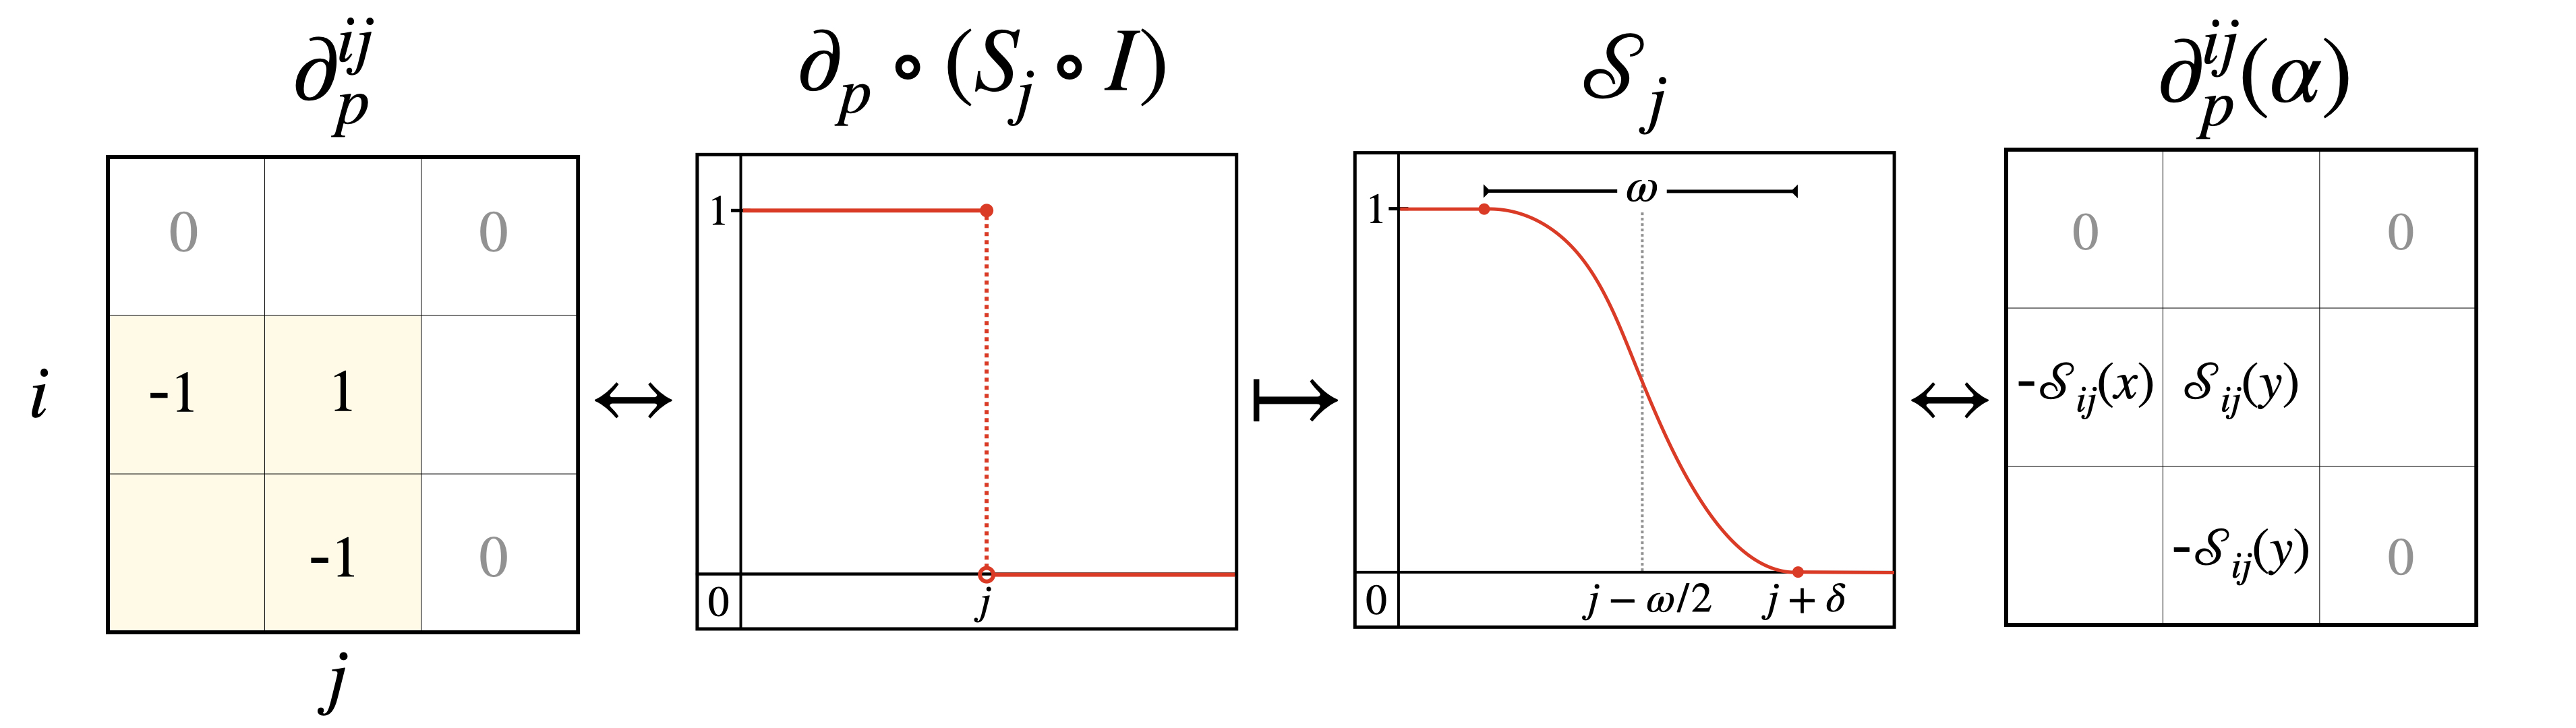
\includegraphics[width=0.88\textwidth,height=1\textheight]{images/smoothstep_3.jpeg}

}

\end{figure}

\[ 
\boxed{
\partial_p^{i,j}(\alpha) = D_p(\mathcal{S}_i \circ f_\alpha) \circ \partial_p(K_\preceq) \circ D_{p+1}(\mathcal{S}_j \circ f_\alpha) 
}
\]

\textbf{Note}: \(P^T \partial_p^{i,j}(\alpha) P\) has rank
\(= \mathrm{rank}(R_p^{i,j}(\alpha))\) for all
\(\alpha \in \mathbb{R}\).

\marginnote{\begin{footnotesize}

Replacing \(S \mapsto \mathcal{S}\) ensures continuity of
\(\partial_p^{i,j}(\alpha)\)

\end{footnotesize}}

\subsection{\texorpdfstring{Rank Invariances when
\(\mathbb{F} = \mathbb{R}\)}{Rank Invariances when \textbackslash mathbb\{F\} = \textbackslash mathbb\{R\}}}\label{rank-invariances-when-mathbbf-mathbbr}

    

\(\hspace{10em} \mathrm{rank}(A) \triangleq \mathrm{dim}(\mathrm{Im}(A))\)

\(\hspace{10em} \hphantom{\mathrm{rank}(A)} \equiv \mathrm{rank}(A^T) \quad \quad \quad \text{(adjoint)}\)

\(\hspace{10em} \hphantom{\mathrm{rank}(A)} \equiv \mathrm{rank}(A^T A) \quad \quad \; \text{(inner product)}\)

\(\hspace{10em} \hphantom{\mathrm{rank}(A)} \equiv \mathrm{rank}(A A^T) \quad \quad \; \text{(outer product)}\)

\(\hspace{10em} \hphantom{\mathrm{rank}(A)} \equiv \mathrm{rank}(S^{-1}AS) \quad \; \text{(change of basis)}\)

\(\hspace{10em} \hphantom{\mathrm{rank}(A)} \equiv \mathrm{rank}(P^T A P) \quad \; \text{(permutation)}\)

\(\hspace{10em} \hphantom{\mathrm{rank}(A)} \equiv \dots \quad \quad \quad \quad \quad \quad \! \! \text{(many others)}\)

\textbf{Q: Can we exploit some of these to speed up the computation?}

\subsection{Spectral functions}\label{spectral-functions}

\textbf{Relaxation \#2}: Approximate \(\mathrm{rank}\) with
\emph{spectral functions} (Bhatia 2013)

\(\quad\quad\quad\quad \mathrm{rank}(X) = \sum \, \mathrm{sgn}_+(\sigma_i)\)

\(\quad\quad\quad\quad \hphantom{\mathrm{rank}(X)}\approx \sum\limits_{i=1}^n \, \phi(\sigma_i, \tau) \phantom{\int\limits_{-\infty}^x}\)

\(\quad\quad\quad\quad \hphantom{\mathrm{rank}(X)}=\lVert \Phi_\tau(X) \rVert_\ast\)

where \(\quad\quad\) \(X = U \mathrm{Diag}(\mathbf{\sigma})V^T\)

where
\(\quad \phi(x, \tau) \triangleq \int\limits_{-\infty}^x\hat{\delta}(z, \tau) dz\)

where
\(\quad \Phi_\tau(X) \triangleq \sum_{i=1}^n \phi(\sigma_i, \tau) u_i v_i^T\)

::: \{.fragment .fade-in-then-semi-outstyle=``text-align: center''\}

\(\Phi_\tau(X)\) is a \emph{Löwner operator} when \(\phi\) is
\emph{operator monotone} (Jiang and Sendov 2018)

\[ A \succeq B \implies \Phi_\tau(A) \succeq \Phi_\tau(B) \]

Closed-form proximal operators exist when \(\Phi_\tau\) convex (Beck
2017)

Often used in nonexpansive mappings (Bauschke, Combettes, et al. 2011)

:::

\subsection{Spectral functions}\label{spectral-functions-1}

\textbf{Relaxation \#2}: Approximate \(\mathrm{rank}\) with
\emph{spectral functions} (Bhatia 2013)

\[\mathrm{rank}(X) = \sum \, \mathrm{sgn}_+(\sigma_i) \approx \sum \, \phi(\sigma_i, \tau), \quad \quad \phi(x, \tau) \triangleq \int\limits_{-\infty}^x\hat{\delta}(z, \tau) dz\]

\[ \text{ where } \quad \hat{\delta}(x, \tau) = \frac{1}{\nu(\tau)} p\left(\frac{x}{\nu(\tau)}\right), \quad \tau > 0, \quad \nu \text{ inc. }\]

\(\Phi_\tau(X)\) is a \emph{Löwner operator} when \(\phi\) is
\emph{operator monotone} (Jiang and Sendov 2018)

\[ A \succeq B \implies \phi_\tau(A) \succeq \phi_\tau(B) \]

Closed-form proximal operators exist when \(\phi_\tau\) convex + minor
conditions\(^1\)

\marginnote{\begin{footnotesize}

(1) See Beck (2017) and Bauschke, Combettes, et al. (2011) for existence
and optimality conditions.

\end{footnotesize}}

\subsection{Löwner Operators}\label{luxf6wner-operators}

For any smoothed Dirac measure\footnote{Any \(\hat{\delta}\) of the form
  \(\nu(1/\tau) p (z \cdot \nu (1/\tau))\) where \(p\) is a density
  function and \(\nu\) positive and increasing is sufficient.}
\(\hat{\delta}\) and differentiable \emph{operator monotone} function
\(\phi: \mathbb{R}_+ \times \mathbb{R}_{++} \to \mathbb{R}_+\), (Bi,
Han, and Pan 2013) show that:

(\(\tau\)-approximate) \(\vphantom{\hat{\delta}}\)

(Monotone) \(\vphantom{\lVert \phi_{\tau}(X) \rVert_\ast}\)

(Smooth) \(\vphantom{\mathbb{R}_1^{n \times m^{\ast^{\ast}}}}\)

(Explicit) \(\vphantom{\partial \lVert \Phi_\tau(\cdot) \rVert_\ast}\)

\(0 \leq \mathrm{rank}(X) - \lVert \Phi_\tau(X) \rVert_\ast \leq c(\hat{\delta})\)

\(\lVert \Phi_{\tau}(X) \rVert_\ast \geq \lVert \Phi_{\tau'}(X) \rVert_\ast\)
for any \(\tau \leq \tau'\)

Semismooth\footnote{Here \emph{semismooth} refers to the existence of
  directional derivatives} on \(\mathbb{R}^{n \times m}\)
\(\vphantom{\mathbb{R}_1^{n \times m^{\ast^{\ast}}}}\), differentiable
on \(\mathbf{S}_+^m\)

Differential \(\partial \lVert \Phi_\tau(\cdot) \rVert_\ast\) has
closed-form soln.

Function/operator pairs ( \(\Phi_\tau\), \(\Phi_\tau\) ) particular
specializations of \emph{matrix functions}:

\[\Phi_\tau(X) = U \Phi_\tau(\Sigma) V^T\]

Commonly used in many application areas, e.g.~compressed sensing (Li
2014)

\subsection{Interpretation:
Regularization}\label{interpretation-regularization}

Ill-posed linear systems \(Ax = b\) are often solved by ``regularized''
least-squares:

\[
x_\tau^\ast = \argmin\limits_{x \in \mathbb{R}^n} \lVert Ax - b\rVert^2 + \tau \lVert x \rVert_1 
\]

The minimizer is given in closed-form by the regularized pseudo-inverse:

\[
x_\tau^\ast = (A^T A + \tau I)^{-1} A^T b
\]

\begin{figure}

{\centering \includegraphics[width=0.5\textwidth,height=\textheight]{images/lasso.png}

}

\end{figure}

\marginnote{\begin{footnotesize}

Image from: https://thaddeus-segura.com/lasso-ridge/

\end{footnotesize}}

\subsection{Interpretation:
Regularization}\label{interpretation-regularization-1}

Under the appropriate parameters\(^1\) for \(\nu\) and \(p\), \(\phi\)
takes the form:

\[
\phi(x, \tau) = \frac{2}{\tau}\int\limits_{0}^z z \cdot  \big((z/\sqrt{\tau})^2+1\big)^{-2} dz = \frac{x^2}{x^2 + \tau}
\]

The corresponding Löwner operator and its Schatten \(1\)-norm is
given\(^2\) by:

\[
\Phi_\tau(X) = (X^T X + \tau \, I_n)^{-1} X^T X, \quad \quad \lVert \Phi_\tau(X) \rVert_\ast = \sum\limits_{i = 1}^n \frac{\sigma_i(X)^2}{\sigma_i(X)^2 + \tau}
\]

This the { \emph{Tikhonov regularization} } in standard form used in
\(\ell_1\)-regression (LASSO)

\marginnote{\begin{footnotesize}

(1) This \(\phi\) corresponds to setting \(\nu(\tau) = \sqrt{\tau}\) and
\(p(x) = 2x (x^2 + 1)^{-2}\); (2) See Theorem 2 in Zhao (2012).

\end{footnotesize}}

\subsection{Application \#1: Filtration
optimization}\label{application-1-filtration-optimization}

\begin{figure}

\begin{minipage}[b]{0.25\linewidth}

{\centering 

\includegraphics{animations/dgms_vineyards.gif}

}

\end{minipage}%
%
\begin{minipage}[b]{0.50\linewidth}

{\centering 

\includegraphics{images/dgm_opt.png}

}

\end{minipage}%
%
\begin{minipage}[b]{0.25\linewidth}

{\centering 

\includegraphics{animations/complex_plain.gif}

}

\end{minipage}%

\end{figure}

\[ 
\alpha^\ast = \argmax_{\alpha \in \mathbb{R}} \; \mathrm{card}\big(\, \left.\mathrm{dgm}(K_\bullet, \, f_\alpha) \right|_{R} \, \big) 
\]

\subsection{Application \#1: Filtration
optimization}\label{application-1-filtration-optimization-1}

\begin{figure}

\begin{minipage}[b]{0.67\linewidth}

{\centering 

\includegraphics{images/codensity_mult.png}

}

\end{minipage}%
%
\begin{minipage}[b]{0.33\linewidth}

{\centering 

\includegraphics{images/optimal_codensity_complex.png}

}

\end{minipage}%

\end{figure}

\[ 
\alpha^\ast = \argmax_{\alpha \in \mathbb{R}} \; \mathrm{card}\big(\, \left.\mathrm{dgm}(K_\bullet, \, f_\alpha) \right|_{R} \, \big) 
\]

\subsection{Application \#1: Filtration
optimization}\label{application-1-filtration-optimization-2}

\begin{figure}

{\centering \includegraphics{images/codensity_ex1.png}

}

\end{figure}

\[ 
    \mu_p^{R} = 
    \mathrm{rank}\begin{bmatrix} \partial_{p+1}^{j + 1, k} & 0 \\
    0 & \partial_{p+1}^{i + 1, l}
    \end{bmatrix}
    - 
    \mathrm{rank}\begin{bmatrix} \partial_{p+1}^{i + 1, k} & 0 \\
    0 & \partial_{p+1}^{j + 1, l}
    \end{bmatrix}
\]

\subsection{Application \#1: Filtration
optimization}\label{application-1-filtration-optimization-3}

\begin{figure}

{\centering \includegraphics{images/codensity_ex2.png}

}

\end{figure}

\[ 
\mu_p^{R} = 
\mathrm{tr}\begin{bmatrix} \lVert \partial_{p+1}^{j + 1, k} \rVert_\ast & 0 \\
0 & \lVert \partial_{p+1}^{i + 1, l} \rVert_{\ast}
\end{bmatrix}
- 
\mathrm{tr}\begin{bmatrix} \lVert \partial_{p+1}^{i + 1, k} \rVert_\ast & 0 \\
0 & \lVert  \partial_{p+1}^{j + 1, l} \rVert_\ast
\end{bmatrix}
\]

\subsection{Application \#1: Filtration
optimization}\label{application-1-filtration-optimization-4}

\begin{figure}

{\centering \includegraphics{images/codensity_ex3.png}

}

\end{figure}

\[ 
\hat{\mu}_p^{R} = 
\mathrm{tr}\begin{bmatrix} \Phi_\tau(\partial_{p+1}^{j + 1, k}) & 0 \\
0 & \Phi_\tau(\partial_{p+1}^{i + 1, l})
\end{bmatrix}
- 
\mathrm{tr}\begin{bmatrix} \Phi_\tau(\partial_{p+1}^{i + 1, k}) & 0 \\
0 & \Phi_\tau(\partial_{p+1}^{j + 1, l})
\end{bmatrix}
\]

\[\boxed{\text{There exists a positive }\tau^\ast > 0 \text{ such that } \mu_p^R = \lceil \hat{\mu}_p^R \rceil \text{ for all } \tau \in (0, \tau^\ast]}\]

\subsection{Application \#1: Filtration
optimization}\label{application-1-filtration-optimization-5}

\includegraphics{images/combinatorial_explosion.png}\footnote{Xu, Weiyu,
  and Babak Hassibi. ``Precise Stability Phase Transitions for \$\ell\_1
  \$ Minimization: A Unified Geometric Framework.'' IEEE transactions on
  information theory (2011)}

\subsection{Application \#1: Filtration
optimization}\label{application-1-filtration-optimization-6}

\begin{figure}

{\centering \includegraphics{images/codensity_ex4.png}

}

\end{figure}

\[ \mu_p^{R} = \mathrm{tr}\begin{bmatrix} \Phi_\tau(\partial_{p+1}^{j + 1, k}) & 0 \\
0 & \Phi_\tau(\partial_{p+1}^{i + 1, l})
\end{bmatrix}
- 
\mathrm{tr}\begin{bmatrix} \Phi_\tau(\partial_{p+1}^{i + 1, k}) & 0 \\
0 & \Phi_\tau(\partial_{p+1}^{j + 1, l})
\end{bmatrix}
\]

\subsection{Application \#1: Filtration
optimization}\label{application-1-filtration-optimization-7}

\begin{figure}

{\centering \includegraphics{images/codensity_ex5.png}

}

\end{figure}

\[ \mu_p^{R} = \mathrm{tr}\begin{bmatrix} \Phi_\tau(\partial_{p+1}^{j + 1, k}) & 0 \\
0 & \Phi_\tau(\partial_{p+1}^{i + 1, l})
\end{bmatrix}
- 
\mathrm{tr}\begin{bmatrix} \Phi_\tau(\partial_{p+1}^{i + 1, k}) & 0 \\
0 & \Phi_\tau(\partial_{p+1}^{j + 1, l})
\end{bmatrix}
\]

Similar to the Iterative Soft-Thresholding Algorithm (ISTA) (Beck 2017)

\subsection{Combinatorial Laplacian}\label{combinatorial-laplacian}

\textbf{Relax \#3:} Replace \(\partial \mapsto L\) with
\emph{combinatorial Laplacians} (Horak and Jost 2013):

\[ \Delta_p = \underbrace{\partial_{p+1} \partial_{p+1}^T}_{L_p^{\mathrm{up}}}  + \underbrace{\partial_{p}^T \partial_{p}}_{L_p^{\mathrm{dn}}} \]

\(f_\alpha\) is 1-to-1 correspondence with inner products on cochain
groups \(C^p(K, \mathbb{R})\)

\[L_p^{i,j}(\alpha) \Leftrightarrow \langle \; f,\, g \; \rangle_{\alpha} \; \text{ on } \;  C^{p+1}(K, \mathbb{R})\]

Benefits: Symmetric, positive semi-definite, have ``nice'' linear and
quadratic forms: \[
L_p^{\text{up}}(\tau, \tau')= \begin{cases}
         \mathrm{deg}_f(\tau) \cdot f^{+/2}(\tau) & \text{ if } \tau = \tau' \\ 
%       \mathrm{deg}(\tau_i) & \text{ if } i = j \\ 
        s_{\tau, \tau'} \cdot  f^{+/2}(\tau) \cdot f(\sigma) \cdot f^{+/2}(\tau') & \text{ if } \tau \overset{\sigma}{\sim} \tau' \\
        0 & \text{ otherwise} 
    \end{cases}
\]

\(\implies\) can represent operator in ``matrix-free'' fashion

\subsection{Interpretation: Diffusion}\label{interpretation-diffusion}

Diffusion processes on graphs often modeled as time-varying
\(v^{(t)} \in \mathbb{R}^n\) via:

\[ v'^{(t)} = -L v^{(t)} \quad \Leftrightarrow \quad L \cdot u(x,t) = - \frac{\partial u(x, t)}{\partial t} \]

\begin{figure}

\begin{minipage}[c]{0.31\linewidth}

{\centering 

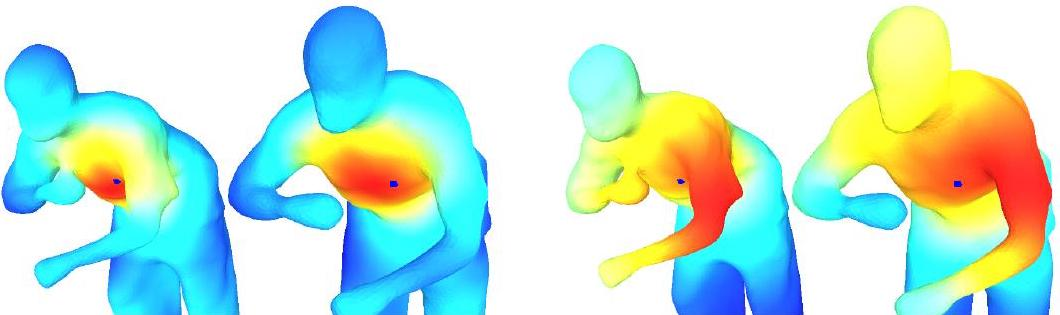
\includegraphics[width=2.60417in,height=\textheight]{images/heat_diffusion.png}

}

\end{minipage}%
%
\begin{minipage}[c]{0.69\linewidth}

{\centering 

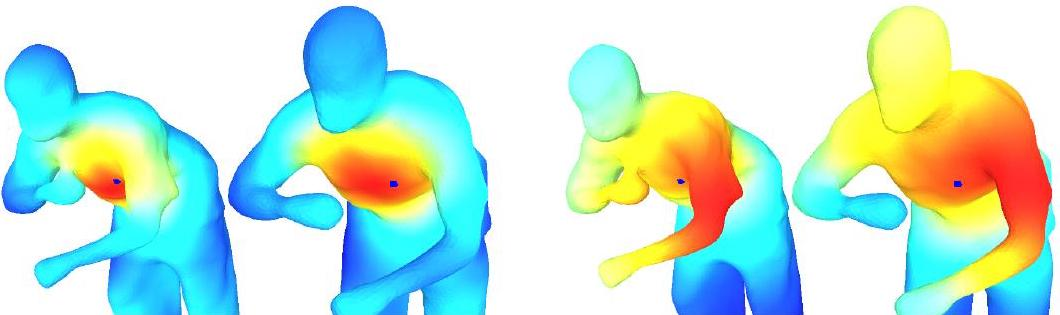
\includegraphics[width=5.72917in,height=\textheight]{images/heat_diffusion.jpg}

}

\end{minipage}%

\end{figure}

Value of \(v(t)\) at time \(t\) given by the \emph{Laplacian exponential
diffusion kernel}:

\[v^{(t)} = \mathrm{exp}(-t L) v^{(0)}\]

\marginnote{\begin{footnotesize}

Images from Crane, Weischedel, and Wardetzky (2017) and Sharma et al.
(2011)

\end{footnotesize}}

\subsection{Interpretation: Diffusion}\label{interpretation-diffusion-1}

Under the appropriate parameters for \(\nu\) and \(\rho\)\footnote{This
  \(\phi\) corresponds to setting \(\nu(\tau) = \tau\) and
  \(p(x) = \mathrm{exp}(-x)\) for \(x > 0\) and \(p(x) = 0\) otherwise},
\(\phi\) takes the form:

\[
\phi(x, \tau) = 1 - \mathrm{exp}(- x / \tau)
\]

The corresponding Löwner operator and its Schatten \(1\)-norm is given
by (for \(t = \tau^{-1}\)):

\[
\Phi_\tau(X) \simeq U \mathrm{exp}(-t \Lambda) U^T, \quad \lVert \Phi_\tau(X) \rVert_\ast \simeq \sum\limits_{i = 1}^n \mathrm{exp}(-t \cdot \lambda_i)
\]

This is the { \emph{Heat kernel} } and its Schatten-1 norm is the {
\emph{heat kernel trace} }

\subsection{Application \#2: Directional
Transform}\label{application-2-directional-transform}

Consider filtering a fixed \(K\) embedded in \(R^d\) by a 1-parameter
directions in \(S^{d-1}\)

\[
K_\bullet = K(v)_i = \{\, x \in X \mid \langle x, v \rangle \leq i  \,\}
\]

\begin{figure}

{\centering \includegraphics[width=3.64583in,height=1\textheight]{animations/dt_single.gif}

}

\end{figure}

\subsection{Application \#2: Directional
Transform}\label{application-2-directional-transform-1}

\[
K_\bullet = K(v)_i = \{\, x \in X \mid \langle x, v \rangle \leq i  \,\}
\]

\begin{figure}

{\centering \includegraphics[width=5.72917in,height=1\textheight]{animations/ph_transform.gif}

}

\end{figure}

\[\{ \; \mathrm{dgm}(v) : v \in S^{d-1} \; \} \Leftrightarrow \text{Persistent Homology Transform (PHT)}\]

Turner et al.\(^1\) show PHT(X) is injective, sparking an inverse theory
for persistence!

\marginnote{\begin{footnotesize}

(1): Turner, Mukherjee, and Boyer (2014)

\end{footnotesize}}

\subsection{Application \#2: Directional
Transform}\label{application-2-directional-transform-2}

Injectivity of the PHT \(\implies\) can impose metric \(\mathcal{D}\)
over { \emph{shape space} } by integrating \(d_B\):

\[ \mathcal{D}(X, Y) \triangleq \sum_{p=0}^d \int_{S^{d-1}} \operatorname{d}_B\left(\mathrm{dgm}_p(X, v) \right), \left( \mathrm{dgm}_p(Y, v) \right) dv \]

To make \(\mathcal{D}(\cdot, \cdot)\) blind to rotations,
Turner\footnote{Turner, Mukherjee, and Boyer (2014)} minimize
\(\mathcal{D}\) over rotations \(\{R_i\}_{i=1}^m\):

\[ d_{\mathrm{PHT}}(X, Y) = \inf_{i = 1, \dots, m} \mathcal{D}(X, R_i(Y)) \]

When \(m = \lvert V \rvert\), computing \(d_{\mathrm{PHT}}(X, Y)\)
requires:

Computing \(\mathrm{dgm}_p(\cdot, v)\) for \(\{X,Y\}\) over sufficiently
dense \(\mathcal{V} \subset S^{d-1}\) (
\({\color{orange} O(m \cdot N^3)}\) )

Minimizing \(\mathcal{D}\) over all \(m\) rotations (
\({\color{red}\approx O(m^2 \cdot N^{1.5} \log N)}\) )\(^1\)

\marginnote{\begin{footnotesize}

(1) Assumes \(d_B \sim O(n^{1.5} \log n)\), following (Kerber, Morozov,
and Nigmetov 2017).

\end{footnotesize}}

\subsection{Application \#2: Directional
Transform}\label{application-2-directional-transform-3}

\begin{figure}

\begin{minipage}[t]{0.30\linewidth}

{\centering 

\raisebox{-\height}{

\includegraphics{animations/dt_single.gif}

}

}

\end{minipage}%
%
\begin{minipage}[t]{0.70\linewidth}

{\centering 

\raisebox{-\height}{

\includegraphics{animations/trace_summary.gif}

}

}

\end{minipage}%

\end{figure}

When \(m = \lvert V \rvert\), computing \(d_{\mathrm{DT}}(X, Y)\)
\(\xcancel{d_{\mathrm{PHT}}(X, Y)}\) requires:

Computing \(\mathrm{tr}(\phi_\tau(\cdot))\) for \(\{X,Y\}\) over
sufficiently dense \(\mathcal{V} \subset S^{d-1}\)
(\(\approx {\color{blue} O(m \cdot N^2)}\))

Phase-aligning two \emph{periodic} signals via FFT (
\({\color{green} O(m \log m)}\) )

\subsection{Application \#2: Directional
Transform}\label{application-2-directional-transform-4}

\begin{figure}

{\centering 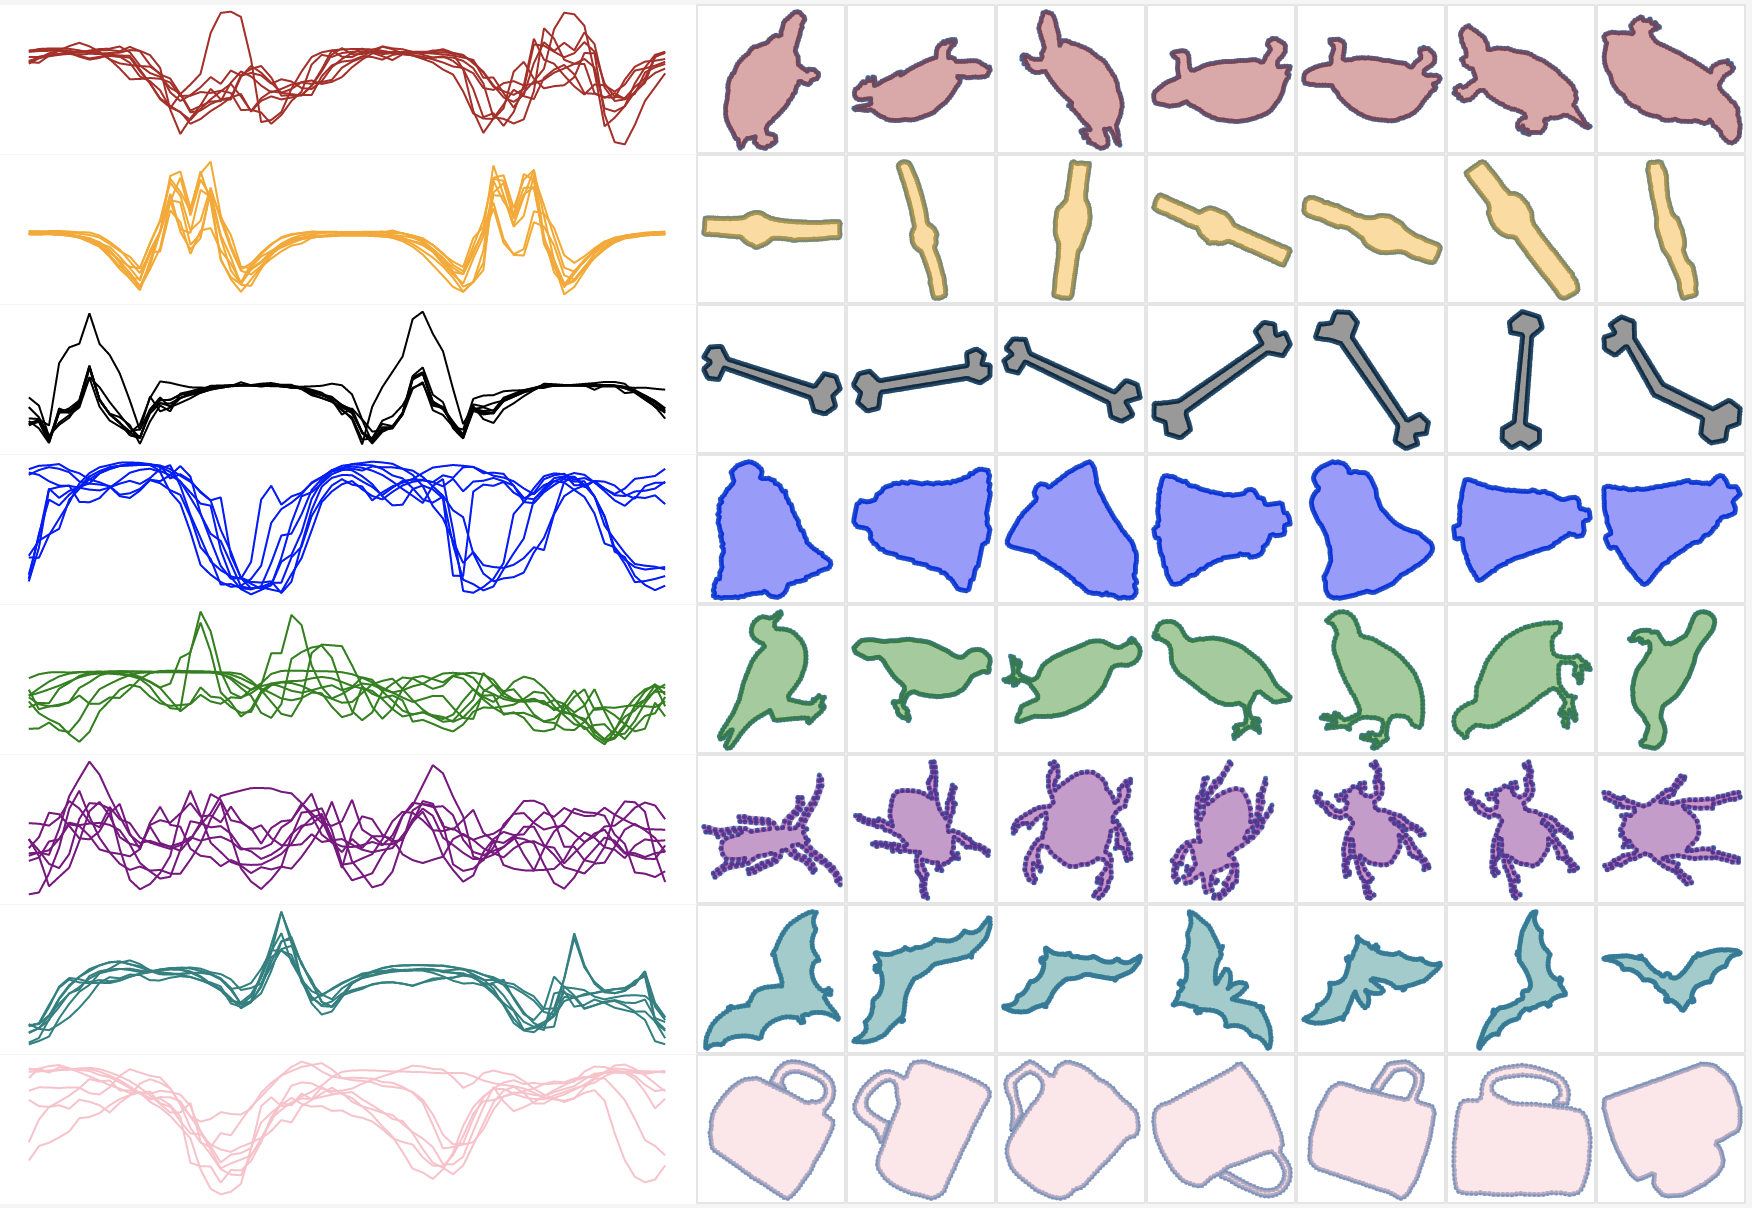
\includegraphics[width=8.85417in,height=1\textheight]{images/shape_signatures.png}

}

\end{figure}

\subsection{Overview}\label{overview-1}

Introduction

Rank duality

Bypassing diagrams

Technical observations

Spectral rank relaxation

Parameterizing \(C(K, \mathbb{R})\)

Spectral functions

Variational interpretations + examples

Computation

Lanczos Iteration

Stochastic trace estimation

Scalability

\subsection{Computation in quadratic
time}\label{computation-in-quadratic-time}

Computing \(A = U \Lambda U^T\) for any \(A \in \mathbf{S}_+^n\) bounded
by \(\Theta(n^3)\) time and \(\Theta(n^2)\) space\footnote{Assumes the
  standard matrix multiplication model for simplicity (i.e.~excludes the
  Strassen-family)}

However, if \(v \mapsto Av \approx O(n)\), then \(\Lambda(A)\)
obtainable in { \(O(n^2)\) time } and {\(O(n)\) space}!

\textbf{Idea}: For some random \(v \in \mathbb{R}^n\), expand successive
powers of \(A\):

\[ 
\begin{align}
K_j &= [ v \mid Av \mid A^2 v \mid \dots \mid A^{j-1}v] && \\
Q_j &= [ q_1, q_2, \dots, q_j] \gets \mathrm{qr}(K_j) && \\
T_j &= Q_j^T A Q_j &&
\end{align}
\]

It turns out that every \(A \in \mathbf{S}\) expanded this way admits a
\emph{three-term recurrence}

\[ A q_j = \beta_{j-1} q_{j-1} + \alpha_j q_j + \beta_j q_{j+1} \]

This is the renowned \emph{\textbf{Lanczos method}} for Krylov subspace
expansion

\subsection{Lanczos iteration}\label{lanczos-iteration}

\begin{figure}

{\centering \includegraphics[width=0.75\textwidth,height=1\textheight]{animations/lanczos_krylov.gif}

}

\end{figure}

\textbf{Theorem (Simon 1984)}: Given a symmetric rank-\(r\) matrix
\(A \in \mathbb{R}^{n \times n}\) whose matrix-vector operator
\(A \mapsto A x\) requires \(O(\eta)\) time and \(O(\nu)\) space, the
Lanczos iteration computes
\(\Lambda(A) = \{ \lambda_1, \lambda_2, \dots, \lambda_r \}\) in
\(O(\max\{\eta, n\}\cdot r)\) time and \(O(\max\{\nu, n\})\) space
\emph{when executed in exact arithmetic}.

\subsection{Randomized trace
approximation}\label{randomized-trace-approximation}

Let \(A = \mathbb{R}^{n \times n}\). If \(v \in \mathbb{R}^n\) a
\(\mathrm{r.v.}\) with \(\mathbb{E}[vv^T] = I\), then:

\[ \mathtt{tr}(A) = \mathtt{tr}(A \mathbb{E}[v v^T]) \quad\quad \text{(identity)} \]

\[ \hphantom{\mathtt{tr}(A)} = \mathbb{E}[\mathtt{tr}(Avv^T)] \quad\quad \text{(linearity)} \]

\[ \hphantom{\mathtt{tr}(A)} = \mathbb{E}[\mathtt{tr}(v^T A v)] \quad\quad \text{(cylic)}\]

\[ \hphantom{\mathtt{tr}(A)} = \mathbb{E}[v^T A v] \quad\quad \text{(symmetry)}\]

\[
\implies \mathtt{tr}(A) \approx \frac{1}{n_v}\sum\limits_{i=1}^{n_v} v_i^\top A v_i, \quad \text{ for } v_i \sim \mathcal{N}(\mu=0, \sigma = 1)
\]

\subsection{Randomized trace
approximation}\label{randomized-trace-approximation-1}

\textbf{Theorem (Ubaru, Chen, and Saad 2017)}: For any \(A \in S_+^n\),
if \(n_v \geq (6/\epsilon^2) \log(2/\eta)\) unit-norm
\(v \in \mathbb{R}^n\) are drawn uniformly from \(\{-1, +1\}^n\), then
for any \(\epsilon, \eta \in (0,1)\):
\[ \mathrm{Pr}\bigg(\lvert \mathrm{tr}_{n_v}(A) - \mathrm{tr}(A) \rvert \leq \epsilon \cdot \mathrm{tr}(A) \bigg) \geq 1 - \eta\]

\(\implies\) Generalizes to \emph{spectral functions} \(\Phi_\tau(X)\)
via \textbf{stochastic Lanczos quadrature}\(^1\)

\[ \mathrm{tr}(\Phi_\tau(X)) \approx \frac{n}{n_v} \bigg( e_1^T \, \Phi_{\tau}(T) \, e_1 \bigg ), \quad \quad T = \mathrm{Lanczos}(X) \]

\[\implies \hat{\mu}_p^{R} \sim O(n \cdot s l^2)^{1} \text{ time and } O(n) \text{ space }\]

Where \(n \sim \lvert K^p \rvert\), and both \(l, s \sim O(1)\) are
small constants\(^2\)

\marginnote{\begin{footnotesize}

(1) See Ubaru, Chen, and Saad (2017). (2) We found setting the lanczos
polynomial degree \(l \leq 20\) and number of Monte-carlo iterations
\(s \leq 200\) was sufficient for most applications.

\end{footnotesize}}

\subsection{\texorpdfstring{Scalability: \(\mathrm{matvecs}\)'s are all
you
need}{Scalability: \textbackslash mathrm\{matvecs\}'s are all you need}}\label{scalability-mathrmmatvecss-are-all-you-need}

\begin{figure}

{\centering \includegraphics[width=7.8125in,height=1\textheight]{images/imate_trace_bench.png}

}

\end{figure}

Figure taken from the new \texttt{imate} package documentation
(\href{https://ameli.github.io/imate/index.html}{\texttt{{[}gh{]}/ameli/imate}})

\subsection{\texorpdfstring{Application \#3: Computing
\(\mathrm{dgm}\)'s}{Application \#3: Computing \textbackslash mathrm\{dgm\}'s}}\label{application-3-computing-mathrmdgms}

\begin{figure}

\begin{minipage}[b]{0.50\linewidth}

{\centering 

\includegraphics[width=4.16667in,height=\textheight]{images/divide_conquer_dgm.png}

}

\end{minipage}%
%
\begin{minipage}[b]{0.50\linewidth}

{\centering 

\includegraphics[width=4.16667in,height=\textheight]{images/bisection_tree.png}

}

\end{minipage}%

\end{figure}

\textbf{Theorem (Chen and Kerber 2011)}: For a simplicial complex \(K\)
of size \(\lvert K \rvert = n\), computing the \(\Gamma\)-persistent
pairs requires \(O(C_{(1-\delta)\Gamma}\mathrm{R}(n) \log n)\) time and
\(O(n + \mathrm{R}(n))\) space, where \(R(n)\) (\(R_S(n)\)) is the time
(space) complexity of computing the rank of a \(n \times n\) boundary
matrix.

\subsection{Other applications (time
permitting)}\label{other-applications-time-permitting}

\begin{figure}

{\centering \includegraphics[width=0.5\textwidth,height=0.9\textheight]{images/dw_chi_comp.png}

}

\end{figure}

\begin{figure}

{\centering \includegraphics[width=0.8\textwidth,height=1\textheight]{images/elephant_sparsify.png}

}

\end{figure}

\subsection{Acknowledgements \&
Advertising}\label{acknowledgements-advertising}

\begin{itemize}
\tightlist
\item
  Explicit proof of (unfactored) \(\beta_p^{\ast}\) in CT book by Tamal
  Dey \& Yusu Wang
\item
  Expression + PH algorithm involving \(\mu_p^\ast\) by Chao Chen \&
  Michael Kerber
\item
  Insightful developments by
  (Bauer\textbar Masood\textbar Giunti\textbar Houry\textbar Kerber\textbar Rathod)
\item
  SLQ due to Ubaru, Chen, and Saad (2017); code ported from
  \href{https://ameli.github.io/imate/}{imate}
\end{itemize}

To see the code develop and track its progress, head to:

\href{https://github.com/peekxc}{{[}gh{]}/peekxc} or
\href{https://mattpiekenbrock.com/}{mattpiekenbrock.com}

Thanks for listening!

\subsection{References}\label{references}

\phantomsection\label{refs}
\setlength{\cslentryspacing}{0em}
\begin{CSLReferences}
\bibitem[\citeproctext]{ref-adams2017persistence}
Adams, Henry, Tegan Emerson, Michael Kirby, Rachel Neville, Chris
Peterson, Patrick Shipman, Sofya Chepushtanova, Eric Hanson, Francis
Motta, and Lori Ziegelmeier. 2017. {``Persistence Images: A Stable
Vector Representation of Persistent Homology.''} \emph{Journal of
Machine Learning Research} 18.

\bibitem[\citeproctext]{ref-anderson1969series}
Anderson Jr, William N, and Richard James Duffin. 1969. {``Series and
Parallel Addition of Matrices.''} \emph{Journal of Mathematical Analysis
and Applications} 26 (3): 576--94.

\bibitem[\citeproctext]{ref-bauer2022keeping}
Bauer, Ulrich, Talha Bin Masood, Barbara Giunti, Guillaume Houry,
Michael Kerber, and Abhishek Rathod. 2022. {``Keeping It Sparse:
Computing Persistent Homology Revised.''} \emph{arXiv Preprint
arXiv:2211.09075}.

\bibitem[\citeproctext]{ref-bauschke2011convex}
Bauschke, Heinz H, Patrick L Combettes, et al. 2011. \emph{Convex
Analysis and Monotone Operator Theory in Hilbert Spaces}. Vol. 408.
Springer.

\bibitem[\citeproctext]{ref-beck2017first}
Beck, Amir. 2017. \emph{First-Order Methods in Optimization}. SIAM.

\bibitem[\citeproctext]{ref-ben1967geometry}
Ben Israel, Adi. 1967. {``On the Geometry of Subspaces in Euclidean
n-Spaces.''} \emph{SIAM Journal on Applied Mathematics} 15.

\bibitem[\citeproctext]{ref-ben2015projectors}
Ben-Israel, Adi. 2015. {``Projectors on Intersection of Subspaces.''}
\emph{Contemporary Mathematics} 636: 41--50.

\bibitem[\citeproctext]{ref-bhatia2013matrix}
Bhatia, Rajendra. 2013. \emph{Matrix Analysis}. Vol. 169. Springer
Science \& Business Media.

\bibitem[\citeproctext]{ref-bi2013approximation}
Bi, Shujun, Le Han, and Shaohua Pan. 2013. {``Approximation of Rank
Function and Its Application to the Nearest Low-Rank Correlation
Matrix.''} \emph{Journal of Global Optimization} 57 (4): 1113--37.

\bibitem[\citeproctext]{ref-boissonnat2014simplex}
Boissonnat, Jean-Daniel, and Clément Maria. 2014. {``The Simplex Tree:
An Efficient Data Structure for General Simplicial Complexes.''}
\emph{Algorithmica} 70: 406--27.

\bibitem[\citeproctext]{ref-bubenik2020persistence}
Bubenik, Peter. 2020. {``The Persistence Landscape and Some of Its
Properties.''} In \emph{Topological Data Analysis: The Abel Symposium
2018}, 97--117. Springer.

\bibitem[\citeproctext]{ref-cerri2013betti}
Cerri, Andrea, Barbara Di Fabio, Massimo Ferri, Patrizio Frosini, and
Claudia Landi. 2013. {``Betti Numbers in Multidimensional Persistent
Homology Are Stable Functions.''} \emph{Mathematical Methods in the
Applied Sciences} 36 (12): 1543--57.

\bibitem[\citeproctext]{ref-chazal2009gromov}
Chazal, Frédéric, David Cohen-Steiner, Leonidas J Guibas, Facundo
Mémoli, and Steve Y Oudot. 2009. {``Gromov-Hausdorff Stable Signatures
for Shapes Using Persistence.''} In \emph{Computer Graphics Forum},
28:1393--403. 5. Wiley Online Library.

\bibitem[\citeproctext]{ref-chazal2016structure}
Chazal, Frédéric, Vin De Silva, Marc Glisse, and Steve Oudot. 2016.
\emph{The Structure and Stability of Persistence Modules}. Vol. 10.
Springer.

\bibitem[\citeproctext]{ref-chen2011output}
Chen, Chao, and Michael Kerber. 2011. {``An Output-Sensitive Algorithm
for Persistent Homology.''} In \emph{Proceedings of the Twenty-Seventh
Annual Symposium on Computational Geometry}, 207--16.

\bibitem[\citeproctext]{ref-crane2017heat}
Crane, Keenan, Clarisse Weischedel, and Max Wardetzky. 2017. {``The Heat
Method for Distance Computation.''} \emph{Communications of the ACM} 60
(11): 90--99.

\bibitem[\citeproctext]{ref-dey2021computing}
Dey, Tamal K, Woojin Kim, and Facundo Mémoli. 2021. {``Computing
Generalized Rank Invariant for 2-Parameter Persistence Modules via
Zigzag Persistence and Its Applications.''} \emph{arXiv Preprint
arXiv:2111.15058}.

\bibitem[\citeproctext]{ref-dey2022computational}
Dey, Tamal Krishna, and Yusu Wang. 2022. \emph{Computational Topology
for Data Analysis}. Cambridge University Press.

\bibitem[\citeproctext]{ref-edelsbrunner2000topological}
Edelsbrunner, Herbert, David Letscher, and Afra Zomorodian. 2000.
{``Topological Persistence and Simplification.''} In \emph{Proceedings
41st Annual Symposium on Foundations of Computer Science}, 454--63.
IEEE.

\bibitem[\citeproctext]{ref-horak2013spectra}
Horak, Danijela, and Jürgen Jost. 2013. {``Spectra of Combinatorial
Laplace Operators on Simplicial Complexes.''} \emph{Advances in
Mathematics} 244: 303--36.

\bibitem[\citeproctext]{ref-jambulapati2021ultrasparse}
Jambulapati, Arun, and Aaron Sidford. 2021. {``Ultrasparse
Ultrasparsifiers and Faster Laplacian System Solvers.''} In
\emph{Proceedings of the 2021 ACM-SIAM Symposium on Discrete Algorithms
(SODA)}, 540--59. SIAM.

\bibitem[\citeproctext]{ref-jiang2018unified}
Jiang, Tianpei, and Hristo Sendov. 2018. {``A Unified Approach to
Operator Monotone Functions.''} \emph{Linear Algebra and Its
Applications} 541: 185--210.

\bibitem[\citeproctext]{ref-kerber2017geometry}
Kerber, Michael, Dmitriy Morozov, and Arnur Nigmetov. 2017. {``Geometry
Helps to Compare Persistence Diagrams.''} ACM New York, NY, USA.

\bibitem[\citeproctext]{ref-kim2020pllay}
Kim, Kwangho, Jisu Kim, Manzil Zaheer, Joon Kim, Frédéric Chazal, and
Larry Wasserman. 2020. {``Pllay: Efficient Topological Layer Based on
Persistent Landscapes.''} \emph{Advances in Neural Information
Processing Systems} 33: 15965--77.

\bibitem[\citeproctext]{ref-komzsik2003lanczos}
Komzsik, Louis. 2003. \emph{The Lanczos Method: Evolution and
Application}. SIAM.

\bibitem[\citeproctext]{ref-lesnick2015interactive}
Lesnick, Michael, and Matthew Wright. 2015. {``Interactive Visualization
of 2-d Persistence Modules.''} \emph{arXiv Preprint arXiv:1512.00180}.

\bibitem[\citeproctext]{ref-li2014new}
Li, Chengjin. 2014. {``A New Approximation of the Matrix Rank Function
and Its Application to Matrix Rank Minimization.''} \emph{Journal of
Optimization Theory and Applications} 163: 569--94.

\bibitem[\citeproctext]{ref-mccleary2022edit}
McCleary, Alexander, and Amit Patel. 2022. {``Edit Distance and
Persistence Diagrams over Lattices.''} \emph{SIAM Journal on Applied
Algebra and Geometry} 6 (2): 134--55.

\bibitem[\citeproctext]{ref-memoli2012some}
Mémoli, Facundo. 2012. {``Some Properties of Gromov--Hausdorff
Distances.''} \emph{Discrete \& Computational Geometry} 48: 416--40.

\bibitem[\citeproctext]{ref-memoli2022persistent}
Mémoli, Facundo, Zhengchao Wan, and Yusu Wang. 2022. {``Persistent
Laplacians: Properties, Algorithms and Implications.''} \emph{SIAM
Journal on Mathematics of Data Science} 4 (2): 858--84.

\bibitem[\citeproctext]{ref-parlett1995we}
Parlett, Beresford N. 1995. {``Do We Fully Understand the Symmetric
Lanczos Algorithm Yet?''} CALIFORNIA UNIV BERKELEY DEPT OF MATHEMATICS.

\bibitem[\citeproctext]{ref-piekenbrock2021move}
Piekenbrock, Matthew, and Jose A Perea. 2021. {``Move Schedules: Fast
Persistence Computations in Coarse Dynamic Settings.''} \emph{arXiv
Preprint arXiv:2104.12285}.

\bibitem[\citeproctext]{ref-sharma2011topologically}
Sharma, Avinash, Radu Horaud, Jan Cech, and Edmond Boyer. 2011.
{``Topologically-Robust 3D Shape Matching Based on Diffusion Geometry
and Seed Growing.''} In \emph{CVPR 2011}, 2481--88. IEEE.

\bibitem[\citeproctext]{ref-simon1984analysis}
Simon, Horst D. 1984. {``Analysis of the Symmetric Lanczos Algorithm
with Reorthogonalization Methods.''} \emph{Linear Algebra and Its
Applications} 61: 101--31.

\bibitem[\citeproctext]{ref-som2020pi}
Som, Anirudh, Hongjun Choi, Karthikeyan Natesan Ramamurthy, Matthew P
Buman, and Pavan Turaga. 2020. {``Pi-Net: A Deep Learning Approach to
Extract Topological Persistence Images.''} In \emph{Proceedings of the
IEEE/CVF Conference on Computer Vision and Pattern Recognition
Workshops}, 834--35.

\bibitem[\citeproctext]{ref-stathopoulos2007nearly}
Stathopoulos, Andreas, and James R McCombs. 2007. {``Nearly Optimal
Preconditioned Methods for Hermitian Eigenproblems Under Limited Memory.
Part II: Seeking Many Eigenvalues.''} \emph{SIAM Journal on Scientific
Computing} 29 (5): 2162--88.

\bibitem[\citeproctext]{ref-turner2014persistent}
Turner, Katharine, Sayan Mukherjee, and Doug M Boyer. 2014.
{``Persistent Homology Transform for Modeling Shapes and Surfaces.''}
\emph{Information and Inference: A Journal of the IMA} 3 (4): 310--44.

\bibitem[\citeproctext]{ref-ubaru2017fast}
Ubaru, Shashanka, Jie Chen, and Yousef Saad. 2017. {``Fast Estimation of
Tr(f(a)) via Stochastic Lanczos Quadrature.''} \emph{SIAM Journal on
Matrix Analysis and Applications} 38 (4): 1075--99.

\bibitem[\citeproctext]{ref-zhao2012approximation}
Zhao, Yun-Bin. 2012. {``An Approximation Theory of Matrix Rank
Minimization and Its Application to Quadratic Equations.''} \emph{Linear
Algebra and Its Applications} 437 (1): 77--93.

\bibitem[\citeproctext]{ref-zomorodian2004computing}
Zomorodian, Afra, and Gunnar Carlsson. 2004. {``Computing Persistent
Homology.''} In \emph{Proceedings of the Twentieth Annual Symposium on
Computational Geometry}, 347--56.

\end{CSLReferences}

\subsection{Computation}\label{computation}

\begin{itemize}
\tightlist
\item
  Permutation invariance \(\implies\) can optimize memory access of
  \(\mathtt{SpMat}\) operation
\end{itemize}

\begin{itemize}
\tightlist
\item
  Any complex data structure suffices, e.g.~tries\(^2\), combinadics,
  etc\ldots{}
\end{itemize}

\begin{itemize}
\tightlist
\item
  Iterative Krylov methods / Lanczos dominate solving sparse
  systems\(^2\)
\end{itemize}

\begin{itemize}
\tightlist
\item
  Many laplacian preconditioning methods known (Jambulapati and Sidford
  2021)
\end{itemize}

\begin{itemize}
\tightlist
\item
  Nearly optimal algorithms known for SDD (Stathopoulos and McCombs
  2007)
\end{itemize}

\marginnote{\begin{footnotesize}

See Parlett (1995) for an overview of the Lanczos. See (Boissonnat and
Maria 2014) for representing complexes.

\end{footnotesize}}

\subsection{Computation}\label{computation-1}

Preliminary experiments suggest scalability is promising

\includegraphics{images/watts_strogatz_perf.png}

\begin{itemize}
\tightlist
\item
  \(\approx \, \leq 25\) Lanczos vectors to approximate full spectrum at
  any \(\epsilon > 0\)
\item
  \(\implies O(n)\) memory to obtain \(\lVert \cdot \rVert_\ast\) in
  \(O(n^2)\) time (with small constants!)
\item
  Previously computed eigenvectors can be re-used for ``warm restarts''
\end{itemize}

\subsection{Experiment \#1: Directional
Transform}\label{experiment-1-directional-transform}

\begin{figure}

{\centering \includegraphics[width=0.8\textwidth,height=1\textheight]{images/shape_signatures.png}

}

\end{figure}

Luis mentioned modding out rotations and translations adn scale to
compare shapes. We can handle rotations via phase alignment.

Sarah mentioned handling orientation.

\subsection{Permutation Invariance}\label{permutation-invariance}

Consider the setting where \(f_\alpha : \mathbb{R} \to \mathbb{R}^N\) is
an \(\alpha\)-parameterized filter function:

\[ \mu_p^R(\, f_\alpha \, ) = \{ \mu_p^R(K_\bullet^\alpha) : \alpha \in \mathbb{R} \}\]

Difficult to compute \(R_\alpha = \partial_\alpha V_\alpha\) for all
\(\alpha\) as \(K_\bullet = (K, f_\alpha)\) is changing
constantly\ldots{}

\[ \mathrm{rank}(\partial_p(K_\bullet)) \equiv \mathrm{rank}(P^T \partial_p(K) P) \]
\[ \mathrm{rank}(\partial_p(K_\bullet)) \equiv \mathrm{rank}(W \mathrm{sgn}(\partial_p(K)) W) \]

Thus we may decouple \(f_\alpha\) and \(K\) in the computation:

\[
\begin{align*}
 \mu_p^{R}(K,f_\alpha) &\triangleq \mathrm{rank}\big(\,\hat{\partial}_{q}^{j + \delta, k}\,\big) - \; \dots \; + \mathrm{rank}\big(\, \hat{\partial}_{q}^{i + \delta, l}\,\big)  \\
&\equiv \mathrm{rank}\big(\,V_p^j \circ \partial_{q} \circ W_q^k \,\big) - \; \dots \; + \mathrm{rank}\big(\,V_p^{i+\delta} \circ \partial_{q} \circ W_q^l \,\big)
 \end{align*}
 \]

where the entries of \(V\), \(W\) change continuously w/ \(\alpha\),
while \(\partial_q\) remains \emph{fixed}\ldots{}

\subsection{Spectral functions}\label{spectral-functions-2}

Nuclear norm \(\lVert X \rVert_\ast = \lVert \mathbf{\sigma} \rVert_1\)
often used in sparse minimization problems like \emph{compressive
sensing} due to its convexity in the unit-ball
\(\{A \in \mathbb{R}^{n \times m} : \lVert A \rVert_2 \leq 1 \}\)

\begin{figure}

\begin{minipage}[b]{0.50\linewidth}

{\centering 

\includegraphics[width=3.125in,height=\textheight]{images/l0_l1.png}

}

\end{minipage}%
%
\begin{minipage}[b]{0.50\linewidth}

{\centering 

\includegraphics[width=3.33333in,height=\textheight]{images/convex_envelope.png}

}

\end{minipage}%

\end{figure}

\textbf{Left:} The \(\ell_0\) and \(\ell_1\) norms on the interval
\([-1,1]\)

\textbf{Right:} \(g\) forms the convex envelope of \(f\) in the interval
\([a,b]\)

\subsection{Spectral functions}\label{spectral-functions-3}

Unfortunately, \(\lVert \cdot \rVert_\ast\) often a poor substitute for
rank

\begin{figure}

{\centering \includegraphics[width=0.7\textwidth,height=1\textheight]{images/rank_relax.png}

}

\end{figure}

\textbf{Left:} The \(\ell_0\) and \(\ell_1\) norms on the interval
\([-1,1]\) \textbf{Right:}

\subsection{Experiment \#2: Intrinsic
signatures}\label{experiment-2-intrinsic-signatures}

\textbf{Dataset:} 3D meshes of animals in different poses (Chazal et al.
2009)

\begin{figure}

{\centering \includegraphics[width=4.42708in,height=1\textheight]{images/gh_data_pose.png}

}

\end{figure}

\textbf{Challenge:} Recognize intrinsic shape categories (via a distance
metric)

\subsection{Experiment \#2: Intrinsic
signatures}\label{experiment-2-intrinsic-signatures-1}

The \emph{Gromov-Hausdorff} distance yields a metric on the set of
compact metric spaces \(\mathcal{X}\)

\[
d_{GH}(d_X, d_Y) = \sup_{x \in X, y \in Y} \lvert d_X(x, \psi(y)) - d_Y(y, \phi(x))\rvert 
\]

\begin{figure}

{\centering \includegraphics[width=6.25in,height=1\textheight]{images/camel_gh.png}

}

\end{figure}

Using intrinsic metric makes \(d_{\mathrm{GH}}\) blind to e.g.~shapes
represented in different \emph{poses}

Unfortunately, the GH distance is NP-hard to compute (Mémoli 2012)

\subsection{Experiment \#2: Intrinsic
signatures}\label{experiment-2-intrinsic-signatures-2}

It's known \(d_B\) (\(d_W\)) on Rips filtrations \(\mathcal{R}(X, d_X)\)
lower bound GH (GW) distance

\[ 
d_B(\mathrm{dgm}_p(\mathcal{R}(X, d_X)), \mathrm{dgm}_p(\mathcal{R}(Y, d_Y))) \; \leq \; d_{GH}((X, d_X), (Y, d_Y))
\]

\begin{figure}

\begin{minipage}[t]{\linewidth}

{\centering 

\raisebox{-\height}{

\includegraphics[width=9.11458in,height=\textheight]{images/camel_gh_rips_comparison.png}

}

}

\end{minipage}%

\end{figure}

Motivates use of persistence in metric settings for e.g.~shape
classification!

\subsection{Experiment \#2: Intrinsic
signatures}\label{experiment-2-intrinsic-signatures-3}

\textbf{Issue:} Diagrams are far from injective, cannot distinguish
e.g.~stretched shapes

\begin{figure}

{\centering \includegraphics[width=5.98958in,height=1\textheight]{images/dgm_noninjective.png}

}

\end{figure}

The lower bound on \(d_{\mathrm{GH}}\) could be totally useless!

\subsection{Experiment \#2: Intrinsic
signatures}\label{experiment-2-intrinsic-signatures-4}

Lower bounds extend to Rips filtrations \emph{augmented} with
real-valued functions \(f, g\):

\[
\mathcal{R}(f) \triangleq \mathcal{R}(X, d_X, f) = \{\mathcal{R}_\alpha(X_\alpha)\}_{\alpha > 0}, \quad X_\alpha \triangleq f^{-1}((-\infty, \alpha)) \subseteq X
\]

The diagrams from \(\mathcal{R}(\lambda \cdot f_X)\) represent
\emph{stable signatures} for each \(\lambda > 0\):

\[
d_B(\mathcal{R}(\lambda \cdot f_X), \mathcal{R}(\lambda \cdot f_Y)) \leq \max(1, \lambda L) \cdot d_{\mathrm{GH}}(X, Y)
\]

Chazal showed these bounds extend to metrics on \emph{augmented} metric
spaces:

\[
\mathcal{X}_1 = \{ (X, d_X, f_X) \mid (X, d_X, f_X) \in \mathcal{X}, f_X: X \to \mathbb{R} \text{ continuous }\}
\]

These signatures also extend to measure metric spaces, see (Chazal et
al. 2009)

{ NOTE: } Size of \(L\) depends on the choice of \(f\) + each
\(\lambda\) produces a new signature!

\subsection{Experiment \#2: Intrinsic
signatures}\label{experiment-2-intrinsic-signatures-5}

\textbf{Ex:} The \emph{eccentricity} function
\(e_X^1(x) = \max_{x' \in X} d_X(x,x')\) has \(L = 2\)

\begin{figure}

{\centering \includegraphics[width=8.07292in,height=1\textheight]{images/dgm_noninjective2.png}

}

\end{figure}

Augmenting via a fraction of \(e_X^1\) modifies the diagrams of the
ellipsoid significantly

\subsection{Experiment \#2: Intrinsic
signatures}\label{experiment-2-intrinsic-signatures-6}

Lower bounds extend to Rips filtrations \emph{augmented} with
real-valued functions \(f, g\):

\[
d_B(\mathcal{R}(\lambda \cdot f_X), \mathcal{R}(\lambda \cdot f_Y)) \leq \max(1, \lambda L) \cdot d_{\mathrm{GH}}(X, Y)
\]

\begin{figure}

\begin{minipage}[t]{0.25\linewidth}

{\centering 

\raisebox{-\height}{

\includegraphics[width=4.6875in,height=\textheight]{images/camel1_rips.png}

}

}

\end{minipage}%
%
\begin{minipage}[t]{0.25\linewidth}

{\centering 

\raisebox{-\height}{

\includegraphics[width=4.6875in,height=\textheight]{images/camel_dgm_rips.png}

}

}

\end{minipage}%
%
\begin{minipage}[t]{0.25\linewidth}

{\centering 

\raisebox{-\height}{

\includegraphics[width=4.6875in,height=\textheight]{images/camel1_ecc.png}

}

}

\end{minipage}%
%
\begin{minipage}[t]{0.25\linewidth}

{\centering 

\raisebox{-\height}{

\includegraphics[width=4.6875in,height=\textheight]{images/camel_dgm_ecc.png}

}

}

\end{minipage}%

\end{figure}

Larger values of \(\lambda\) yield worse bounds, but can lead to simpler
diagrams

\subsection{Experiment \#2: Intrinsic
signatures}\label{experiment-2-intrinsic-signatures-7}

Each choice of \(\lambda > 0\) yields a \emph{stable signature} via
\(\mathcal{R}(\lambda \cdot f_X)\)

Which value of \(\lambda\) to choose?

\begin{figure}

{\centering \includegraphics[width=9.89583in,height=1\textheight]{images/camel1_interp1.png}

}

\end{figure}

\subsection{Experiment \#2: Intrinsic
signatures}\label{experiment-2-intrinsic-signatures-8}

Each choice of \(\lambda > 0\) yields a \emph{stable signature} via
\(\mathcal{R}(\lambda \cdot f_X)\)

Which value of \(\lambda\) to choose?

\begin{figure}

{\centering \includegraphics[width=9.89583in,height=1\textheight]{images/camel1_interp2.png}

}

\end{figure}

We sample from \(\Delta_+\) randomly, retaining signatures with
sufficient topological activity

\subsection{Experiment \#2: Intrinsic
signatures}\label{experiment-2-intrinsic-signatures-9}

\ldots and compared the computed spectral signatures under the relative
distance metric:

\[
\Lambda(\mu_p^R) = \{\sigma_1, \sigma_2, \dots, \sigma_n \}, \quad \quad \chi(\mathbf{\sigma}, \mathbf{\tilde{\sigma}}) = \sum\limits_{i=1}^n \frac{\lvert \sigma_i - \tilde{\sigma}_i \rvert}{\sqrt{\sigma_i + \tilde{\sigma}_i}}
\]

\begin{figure}

{\centering \includegraphics[width=7.8125in,height=1\textheight]{images/dw_chi_comp.png}

}

\end{figure}

\subsection{Overview}\label{overview-2}



\end{document}
